% !TeX document-id = {5c9b7af7-cc8b-495c-a61c-cd548e104791}
% !TeX TXS-program:compile = txs:///pdflatex/[--shell-escape]

%include guard:
\ifdefined\GlobalAlreadyIncluded
  \expandafter\endinput
\fi

\gdef\GlobalAlreadyIncluded{}
%

\documentclass[accentcolor=3c,landscape,ngerman,presentation,t,usenames,dvipsnames,svgnames,table, aspectratio=169]{tudabeamer}

% Template-Modifikationen
\addtobeamertemplate{frametitle}{}{\vspace{-1em}} % mehr Platz vor dem Inhalt

% andere global gemeinsame definitionen
%Includes
\usepackage[ngerman]{babel} %Deutsche Silbentrennung
\usepackage[utf8]{inputenc} %Deutsche Umlaute
\usepackage{float}
\usepackage{graphicx}
\usepackage{minted}

\DeclareGraphicsExtensions{.pdf,.png,.jpg}

\makeatletter
\author{Vorkursteam der Fachschaft Informatik}
\let\Author\@author

% dark Mode
\ExplSyntaxOn
\RequirePackage{pagecolor,xcolor, graphicx} % Used for dark Mode
\bool_gset_false:N \g_dark_mode_bool % Disable by default
\newcommand{\enableDarkMode}{ %Command to enable Dark Mode (only works before \begin{document})
	\definecolor{anthrazitgrau}{HTML}{293133}
	\pagecolor{anthrazitgrau}
	\color{white}

	\cs_if_exist:NT \setbeamercolor {
		\setbeamercolor*{smallrule}{bg=.}
		\setbeamercolor*{normal~text}{bg=,fg=.}
		\setbeamercolor*{background canvas}{parent=normal~text}
		\setbeamercolor*{section~in~toc}{parent=normal~text}
		\setbeamercolor*{subsection~in~toc}{parent=normal~text,fg=\thepagecolor}
		\setbeamercolor*{footline}{parent=normal~text}
		\setbeamercolor{block~title~alerted}{fg=white,bg=white!20!\thepagecolor}
		\setbeamercolor*{block~body}{bg=white!10!\thepagecolor}
		\setbeamercolor*{block~body~alerted}{bg=\thepagecolor}
	}
	\cs_if_exist:NT \setbeamertemplate {
		\setbeamertemplate{subsection~in~toc~shaded}[default][50]
	}
	\bool_gset_true:N \g_dark_mode_bool
	% Prefer inverted Logo with dark Mode
	% \IfFileExists{tuda_logo_inverted.pdf}{\tl_gset:Nn \g_ptxcd_logofile_tl {tuda_logo_inverted.pdf}}{}
	% \hbox_gset:Nn \g__ptxcd_logo_box {% Update Logo Box
	% 	\makebox[2.2\c_ptxcd_logoheight_dim][l]{\includegraphics[height=\c_ptxcd_logoheight_dim]{\g_ptxcd_logofile_tl}}%
	% }
}

% dark Mode Makros
\prg_new_conditional:Nnn \__ptxcd_if_dark_mode: {T,F,TF} { % Conditional to check if dark Mode is active
	\bool_if:NTF \g_dark_mode_bool
	{\prg_return_true:}
	{\prg_return_false:}
}

\cs_set_eq:NN\IfDarkModeT \__ptxcd_if_dark_mode:T % Easy dark Mode check for use in document
\cs_set_eq:NN\IfDarkModeF \__ptxcd_if_dark_mode:F
\cs_set_eq:NN\IfDarkModeTF \__ptxcd_if_dark_mode:TF

\newcommand{\includeinvertablegraphics}[2][]{% Grafik wird beim Dark Mode automatisch Invertiert (rgb)
	\IfDarkModeTF{\includegraphics[decodearray={1.0~0.0~1.0~0.0~1.0~0.0},#1]{#2}}{\includegraphics[#1]{#2}}
}
\newcommand{\includeinvertablegrayscalegraphics}[2][]{% Grafik wird beim Dark Mode automatisch Invertiert (grayscale)
	\IfDarkModeTF{\includegraphics[decodearray={1.0 0.0},#1]{#2}}{\includegraphics[#1]{#2}}
}

% DARK_MODE environment check (enable if DARK_MODE=1)
\sys_get_shell:nnN { kpsewhich ~ --var-value ~ DARK_MODE } { } \l_dark_mode_env_var_tl
\tl_trim_spaces:N \l_dark_mode_env_var_tl
\tl_if_eq:NnT \l_dark_mode_env_var_tl {1} {\enableDarkMode{}}
\ExplSyntaxOff

% macros
\renewcommand{\arraystretch}{1.2} % Höhe einer Tabellenspalte minimal erhöhen
\newcommand{\N}{{\mathbb N}}
\newcommand{\code}{\inputminted[]{python}}
\newmintedfile[pythonfile]{python}{
	fontsize=\small,
	style=\IfDarkModeTF{fruity}{friendly},
	linenos=true,
	numberblanklines=true,
	tabsize=4,
	obeytabs=false,
	breaklines=true,
	autogobble=true,
	encoding="utf8",
	showspaces=false,
	xleftmargin=20pt,
	frame=single,
	framesep=5pt,
}
\newmintinline{python}{
	style=\IfDarkModeTF{fruity}{friendly},
	encoding="utf8"
}

\definecolor{codegray}{HTML}{eaf1ff}
\newminted[bashcode]{awk}{
	escapeinside=||,
	fontsize=\small,
	style=\IfDarkModeTF{fruity}{friendly},
	linenos=true,
	numberblanklines=true,
	tabsize=4,
	obeytabs=false,
	breaklines=true,
	autogobble=true,
	encoding="utf8",
	showspaces=false,
	xleftmargin=20pt,
	frame=single,
	framesep=5pt
}

\let\origpythonfile\pythonfile
\renewcommand{\pythonfile}[1]{\pythonfileh{#1}{}}
\newcommand{\pythonfileh}[2]{\origpythonfile[#2]{#1}}

\newcommand*{\ditto}{\texttt{\char`\"}}

%Includes
\usepackage{epstopdf}
\usepackage{wrapfig}
\usepackage{tipa}
\usepackage{tikz}
\usetikzlibrary{calc,shapes,arrows}
%tip: use http://l04.scarfboy.com/coding/phonetic-translation?from=ipa&fromtext=%CB%88pa%C9%AA%CE%B8n%CC%A9&to=tipa
%for converting ipa

\graphicspath{ {./media/} }

\def\shortyear#1{\expandafter\shortyearhelper#1}
\def\shortyearhelper#1#2#3#4{#3#4}

\newcount\NextYear
\NextYear = \year
\advance\NextYear by 1

\newcommand\NextYearShort{\shortyear{\the\NextYear}}

% notes
\usepackage{pgfpages}
\setbeamertemplate{note page}[plain]
%\setbeameroption{show notes on second screen}

% macro for change speaker sign
\newcommand{\changespeaker}{
	\begin{tikzpicture}[line width=.6mm, shorten >= 3pt, shorten <= 3pt]

		\coordinate (c1);
		\coordinate[right of=c1] (c2);

		\draw[rectangle, draw=red!80, fill=red!80, align=center, rounded corners] ($(c1.north west)+(0,-0.3)$) rectangle ($(c2.south east)+(0, 0.3)$) {};
		\draw[->,white] (c1)[bend left] to node[auto] {} (c2);
		\draw[->,white] (c2)[bend left] to node[auto] {} (c1);
	\end{tikzpicture}
}

%Listing-Style pyhon
\title[Programmiervorkurs]{Programmiervorkurs Wintersemester \the\year/\NextYearShort}
\subtitle{{\small der Fachschaft Informatik}}
\logo*{
\includegraphics{../globalMedia/bildmarke_ohne_rand}}
\institute{Fachschaft Informatik}
\date{Wintersemester \the\year/\NextYearShort}


% macros
\newcommand{\livecoding}{
		\ifdefined\StreamSlides
			\begin{frame}
				\frametitle{\insertsectionhead \\  {\small \insertsubsectionhead}}\centering \huge 	\vskip 2cm\textbf{\textcolor{red}{Live-Coding}}
			\end{frame}
		\fi
	}

%\newcommand{\slidehead}{\frametitle{\insertsectionhead \\ {\small \insertsubsectionhead}}\vspace{3mm}}
\newcommand{\slidehead}{\frametitle{\insertsectionhead} \framesubtitle{\insertsubsectionhead}\vspace{3mm}}
\newcommand{\tocslide}{\begin{frame}[t]\frametitle{Inhaltsverzeichnis}\vspace{3mm}{\small\tableofcontents[subsectionstyle=shaded]}\end{frame}}

\newcommand{\nextvid}[2]{
	\ifdefined\StreamSlides
	\else
		\section{Nächstes Video}
		\begin{frame}[t]
			\slidehead
			\begin{block}{Nächstes Video}
				\vspace{0.5cm}
				#1
				\vspace{0.5cm}
			\end{block}
			\ifx\hfuzz#2\hfuzz
				\vspace{2.5cm}
			\else
				{\begin{block}{Bonus Video}
					\vspace{0.5cm}
					#2
					\vspace{0.5cm}
				\end{block}}
			\fi
			Danke fürs Zuschauen!\\
			Links zu den Folien und Quellen sind in der Videobeschreibung.
		\end{frame}
	\fi
}


\usepackage{verbatim}
\usetikzlibrary{decorations.pathreplacing}
\usetikzlibrary{shapes.misc}


% colors
\definecolor{lightpetrol}{RGB}{0,223,194}

% dark Mode
\ExplSyntaxOn
\RequirePackage{pagecolor,xcolor, graphicx} % Used for dark Mode
\bool_gset_false:N \g_dark_mode_bool % Disable by default
\newcommand{\enableDarkMode}{ %Command to enable Dark Mode (only works before \begin{document})
	\pagecolor{black}
	\color{white}
	\setbeamercolor*{smallrule}{bg=white}
	\setbeamercolor*{normal~text}{bg=,fg=white}
	\setbeamercolor*{background canvas}{parent=normal~text}
	\setbeamercolor*{section~in~toc}{parent=normal~text}
	\setbeamercolor*{subsection~in~toc}{parent=normal~text,fg=black}
	\setbeamertemplate{subsection~in~toc~shaded}[default][50]
	\setbeamercolor*{footline}{parent=normal~text}
	\setbeamercolor{block~title~alerted}{fg=white,bg=white!20!black}
	\setbeamercolor*{block~body}{bg=white!10!black}
	\setbeamercolor*{block~body~alerted}{bg=black}
	\bool_gset_true:N \g_dark_mode_bool
	\IfFileExists{tuda_logo_inverted.pdf}{\tl_gset:Nn \g_ptxcd_logofile_tl {tuda_logo_inverted.pdf}}{} % Prefer inverted Logo with dark Mode
	\hbox_gset:Nn \g__ptxcd_logo_box {% Update Logo Box
		\makebox[2.2\c_ptxcd_logoheight_dim][l]{\includegraphics[height=\c_ptxcd_logoheight_dim]{\g_ptxcd_logofile_tl}}%
	}
}

% dark Mode Makros
\prg_new_conditional:Nnn \__ptxcd_if_dark_mode: {T,F,TF} { % Conditional to check if dark Mode is active
	\bool_if:NTF \g_dark_mode_bool
	{\prg_return_true:}
	{\prg_return_false:}
}

\cs_set_eq:NN\IfDarkModeT \__ptxcd_if_dark_mode:T % Easy dark Mode check for use in document
\cs_set_eq:NN\IfDarkModeF \__ptxcd_if_dark_mode:F
\cs_set_eq:NN\IfDarkModeTF \__ptxcd_if_dark_mode:TF

\newcommand{\includeinvertablegraphics}[2][]{% Grafik wird beim Dark Mode automatisch Invertiert (rgb)
	\IfDarkModeTF{\includegraphics[decodearray={1.0~0.0~1.0~0.0~1.0~0.0},#1]{#2}}{\includegraphics[#1]{#2}}
}
\newcommand{\includeinvertablegrayscalegraphics}[2][]{% Grafik wird beim Dark Mode automatisch Invertiert (grayscale)
	\IfDarkModeTF{\includegraphics[decodearray={1.0 0.0},#1]{#2}}{\includegraphics[#1]{#2}}
}

% DARK_MODE environment check (enable if DARK_MODE=1)
\sys_get_shell:nnN { kpsewhich ~ --var-value ~ DARK_MODE } { } \l_dark_mode_env_var_tl
\tl_trim_spaces:N \l_dark_mode_env_var_tl
\tl_if_eq:NnT \l_dark_mode_env_var_tl {1} {\enableDarkMode{}}
\ExplSyntaxOff

% notes
\usepackage{pgfpages}
\setbeamertemplate{note page}[plain]
%\setbeameroption{show notes on second screen}

% macro for change speaker sign
\newcommand{\changespeaker}{
	\begin{tikzpicture}[line width=.6mm, shorten >= 3pt, shorten <= 3pt]

		\coordinate (c1);
		\coordinate[right of=c1] (c2);

		\draw[rectangle, draw=red!80, fill=red!80, align=center, rounded corners] ($(c1.north west)+(0,-0.3)$) rectangle ($(c2.south east)+(0, 0.3)$) {};
		\draw[->,white] (c1)[bend left] to node[auto] {} (c2);
		\draw[->,white] (c2)[bend left] to node[auto] {} (c1);
	\end{tikzpicture}
}

%Listing-Style pyhon
\title[Programmiervorkurs]{Programmiervorkurs Wintersemester \the\year/\NextYearShort}
\subtitle{{\small der Fachschaft Informatik}}
\logo*{
\includegraphics{../globalMedia/bildmarke_ohne_rand}}
\institute{Fachschaft Informatik}
\date{Wintersemester \the\year/\NextYearShort}


% macros
\newcommand{\livecoding}{\begin{frame}\frametitle{\insertsectionhead \\  {\small \insertsubsectionhead}}\centering \huge \vskip 2cm\textbf{\textcolor{red}{Live-Coding}}\end{frame}}

%\newcommand{\slidehead}{\frametitle{\insertsectionhead \\ {\small \insertsubsectionhead}}\vspace{3mm}}
\newcommand{\slidehead}{\frametitle{\insertsectionhead} \framesubtitle{\insertsubsectionhead}\vspace{3mm}}
\newcommand{\tocslide}{\begin{frame}[t]\frametitle{Inhaltsverzeichnis}\vspace{3mm}{\small\tableofcontents[subsectionstyle=shaded]}\end{frame}}


% colors
\definecolor{lightpetrol}{RGB}{\IfDarkModeTF{0,136,119}{0,223,194}}

\usepackage{verbatim}
\usetikzlibrary{decorations.pathreplacing}
\usetikzlibrary{shapes.misc}

\begin{document}

%Deckblatt
\begin{titleframe}
	\vspace{3mm}
	\begin{columns}
		\begin{column}{6cm}
			\vspace{4.32mm}
			\begin{center}
				{\huge Einleitung}
			\end{center}
			\begin{figure}
				\centering
				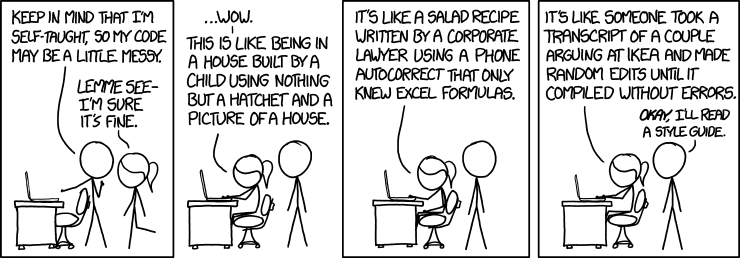
\includegraphics[scale=0.3]{code_quality.png}
				\\	\sffamily \tiny Bild: \href{https://xkcd.com/1513/}{https://xkcd.com/1513/}
			\end{figure}
		\end{column}
		\begin{column}{3.5cm}
			\vspace{-0.3mm}
			\begin{figure}
				\centering
				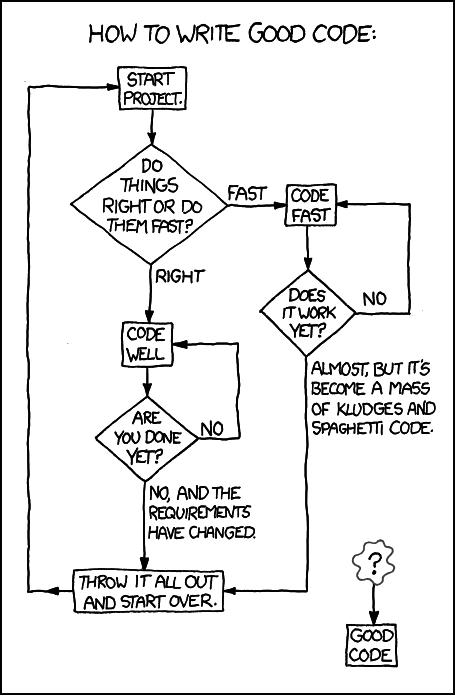
\includegraphics[scale=0.2]{good_code.png}
				\\	\sffamily \tiny Bild: \href{https://xkcd.com/844/}{https://xkcd.com/844/}
			\end{figure}
		\end{column}
	\end{columns}

\end{titleframe}

%Inhaltsverzeichnis
\tocslide

% Um den Vorkurs zu beginnen muss ich irgendwie die Zuschauer für das Programmieren inspirieren. Es muss sie überzeugen, dass Programmieren geil ist, das die Vorträger sympathisch sind und dass eigentlich alles super ist. Dafür mache ich eine Einführung, die Programmieren als Abstraktes Gedankenexperiment einführt.
% Man stelle sich eine außerirdische Lebensform vor, welche eine komplett andere Art von Intelligenz als wir Menschen hat. Wie kann man mit dieser Lebensform kommunizieren. Wir haben verschiedene Informationen über die Lebensform: Sie ist exakt, vergisst keine Details, ist sehr fleißig, ist sehr schnell aber ist nicht eigenständig. Welche Sprache kann man benutzen, bei der sowohl wir Menschen, als auch diese Lebensform etwas versteht. Englisch würde zwar uns Menschen gefallen, aber Englisch hat zu viele Wörter deren genaue Bedeutung unklar ist. "Mehrdeutigkeit" ist etwas mit der die Lebensform überhaupt nicht umgehen kann. Die Lebensform könnte eine Sprache vorschlagen, die nur aus Nullen und Einsen besteht ein so begrenztes Vokabular hat, dass jeder Begriff eine exakte Bedeutung hat. Damit kann der Mensch jedoch schlecht umgehen, weil er sich Zahlen schlecht merken kann und keine Intuition aufbaut was die Begriffe bedeuten. Lösung: Ein Mittelweg: Eine künstlich erfundene Sprache, die eine sehr begrenzte Anzahl Begriffe auf Englisch hat, die man sich gut merken kann und gleichzeitig eine exakt definierte Bedeutung hat, so dass das Wesen sich es auch merken kann.

\section{Warum mit Computer kommunizieren?}
\begin{frame}
	\slidehead
	\begin{itemize}
		\item Computer sind rein-mathematische Maschinen
		\item Computer macht einfache Arbeitsschritte extrem \textbf{schnell}
		\item Programme sind aus vielen Arbeitsschritten zusammengesetzt
		\pythonfile{listings/Programmieren.txt}
	\end{itemize}
\end{frame}

\section{Was tun wir hier eigentlich?}
\begin{frame}
	\slidehead
	\begin{itemize}
		\item Programmieren mit Python \textcolor{gray}{[\textprimstress pa\textsci \texttheta n] [\textprimstress pa\textsci \texttheta \textscripta n]}
		\item Python?
		\pause
		\item[] $\Rightarrow$ Programmiersprache!
		\item[] $\Rightarrow$ Verständlicher für Menschen
		\item[] $\Rightarrow$ Oft verwendet
	\end{itemize}

	\pause
	\vspace{0.75cm}

	\tikzstyle{rect} = [rectangle, rounded corners, minimum width=3cm, minimum height=1cm,text centered, draw=black, fill=red!10]
	\centering
	\begin{tikzpicture}[node distance=5cm]
		\node (syntax) [rect, text width=4cm, minimum height=2cm] {\textbf{Syntax}\\ Wortschatz};
		\node (grammatik) [rect, right of=syntax, text width=4cm, minimum height=2cm] {\textbf{Grammatik}\\ Regeln um Befehle zusammenzusetzen};
	\end{tikzpicture}

\end{frame}

\begin{comment}
	\section{Das erste Programm}
	\subsection{Wie fange ich an?}
	\begin{frame}
		\slidehead
		\begin{itemize}
			\item Befehle bestehen aus Text
			\item Mit einem einfachen Texteditor schreibt man Befehle in eine Datei
			\item Anschließend interpretiert der Computer die Befehle
		\end{itemize}
	\end{frame}
\end{comment}

\subsection{Interpreter?}
\begin{frame}[t]
	\slidehead
	\begin{columns}[T]
		\begin{column}{2cm}
			\begin{tikzpicture}

				\node[] (mensch) at (0,0) {
\includegraphics[height=1.3cm]{media/wesen_notebook.png}};

				\visible<2->{
				\node[fill=lightpetrol,draw, inner sep=5pt,rounded rectangle] (interpreter) at (0,-1.8) {Interpreter};
				\draw[->,line width=.6mm] (mensch.south) -- (interpreter.north);
				}
				\visible<3->{
				\node[fill=lightgray,draw, inner sep=5pt, rounded rectangle] (computer) at (0,-4) {Computer};
				\draw[->,line width=.6mm] (interpreter.south) -- (computer.north);
				}
			\end{tikzpicture}
		\end{column}
		\begin{column}{10cm}
			\begin{itemize}
				\item[]
				\item \textbf{Der Mensch} beschreibt die Aufgabe in einer Programmiersprache $\Rightarrow$ Quelltext
				\item[]
				\item[]
				\visible<2->{
				\item \textbf{Der Interpreter} interpretiert den Quelltext als Maschinenbefehle

				}
				\item[]
				\item[]
				\visible<3->{
				\item \textbf{Der Computer} führt die Maschinenbefehle aus
				}
			\end{itemize}
		\end{column}
	\end{columns}
\end{frame}


\subsection{}
\begin{frame}
	% Beispiel, um zu zeigen wie so ein Befehl aussieht (und ein Kommentar)
	\slidehead
	\hskip .8cm
	\vspace{.5cm}
	\pythonfile{listings/HelloWorld.py}

	\pause

	\vspace{-2.55cm}
	\hskip .8cm
	\begin{tikzpicture}
		\draw [decorate,decoration={brace,amplitude=6pt}]
		(0,0.5) -- (3.7,0.5) node [black,midway,yshift=15pt,xshift=3.4cm] {Kommentar: wird vom Computer \textbf{ignoriert}, ist für Menschen \textbf{nützlich}};
	\end{tikzpicture}

	\pause

	\vspace{1.8cm}
	\hskip .8cm
	\begin{minipage}[b]{0.4\textwidth}
		\begin{tikzpicture}
			\draw [decorate,decoration={mirror,brace,amplitude=6pt}]
			(0,0.5) -- (1,0.5) node [black,midway,yshift=-15pt] {Befehl};
		\end{tikzpicture}
	\end{minipage}
	\pause
	\hskip -3.8cm
	\begin{minipage}[b]{0.4\textwidth}
		\begin{tikzpicture}
			\draw [decorate,decoration={mirror,brace,amplitude=6pt}]
			(1.1,0.5) -- (3.35,0.5) node [black,midway,yshift=-15pt] {Text};
		\end{tikzpicture}
	\end{minipage}

	\pause
	\vspace{0.5cm}
	\begin{block}{Wichtig}
		\begin{itemize}
			\item Text muss in \pythoninline{" "} oder in \pythoninline{' '} stehen
			\item Verwende \textbf{aussagekräftige} Kommentare \footnotesize (dein späteres Ich wird dir danken)!
		\end{itemize}
	\end{block}
\end{frame}


\subsection{Textausgabe}
\begin{frame}
	% Beispiel wie kleinkariert man mit diesem Computer reden muss - unintuitiv für Menschen, dass man nicht einfach "Enter" drücken kann, sondern so kyptisch "\n" schreiben muss
	\slidehead
	\begin{itemize}
		\item Mithilfe des Befehls \pythoninline{print()} kann Text auf der Konsole ausgeben werden
	\end{itemize}
	\begin{columns}
		\begin{column}{6cm}
			\pythonfile{listings/print_Listing.py}
		\end{column}
		\begin{column}{6cm}
			\pythonfile{listings/printSingleLine_Listing.py}
		\end{column}
	\end{columns}

	\begin{block}{Merke}
		\pythoninline{print()} erzeugt einen Zeilenumbruch nach der Ausgabe
	\end{block}
\end{frame}

\subsection{Steuerzeichen}
\begin{frame}
	\slidehead

	\begin{table}[htbp]
		\begin{tabular}{|l|l|}
			\hline
			\textbf{Symbol} & \textbf{Wirkung} \\ \hline
			$\backslash$n & Zeilenumbruch \\ \hline
			$\backslash$\" & Doppeltes Anführungszeichen  (nur in \pythoninline{" "} nötig) \\ \hline
			$\backslash$' & Einfaches Anführungszeichen (nur in \pythoninline{' '} nötig) \\ \hline
			$\backslash \backslash$ & Backslash \\ \hline
		\end{tabular}
		\label{}
	\end{table}

	\pythonfile{listings/Steuerzeichen_Listing.py}
\end{frame}

\section{Vom Quelltext zum fertigen Programm}
\begin{frame}
	\slidehead

	\begin{columns}[T]
		\begin{column}{.3\textwidth}
			\begin{tikzpicture}
				\node[] (mensch) at (0,0) {
\includegraphics[height=1.3cm]{media/wesen_notebook.png}};

				\node[fill=lightpetrol,draw, inner sep=5pt,rounded rectangle] (file) at (0,-1.8) {helloworld.py};
				\draw[->,line width=.6mm] (mensch.south) -- (file.north);

				\node[fill=lightpetrol,draw, inner sep=5pt,rounded rectangle] (python) at (0,-4) {\texttt{python3 helloworld.py}};
				\draw[->,line width=.6mm] (file.south) -- (python.north);
			\end{tikzpicture}
		\end{column}
		\begin{column}{.7\textwidth}
			\begin{itemize}
				\item Mit sinnvollem Dateinamen
				\item Ausführen: \texttt{python3 dateiName.py}
				\item Python-Programme laufen überall, wo Python installiert ist
			\end{itemize}
		\end{column}
	\end{columns}
\end{frame}

\section{Ein Python-Programm schreiben}
\begin{frame}
	\slidehead

	\begin{center}
		\vskip -10 pt
		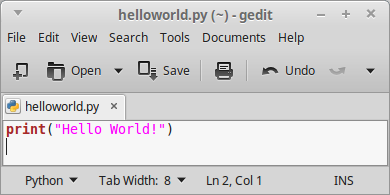
\includegraphics[scale=0.25]{HelloWorldImEditor}
	\end{center}

	\begin{itemize}
		\item Programm wird in einem herkömmlichen Editor geschrieben
		\item Poolraumrechner: \texttt{gedit}, \texttt{atom}, \texttt{kate}
	\end{itemize}
	\begin{alertblock}{Wichtig}
		Verwendet keine Textverarbeitung wie LibreOffice, Pages oder MS Word!
	\end{alertblock}
\end{frame}

\section{Ein Python-Programm ausführen}
\begin{frame}[fragile]
	\slidehead
	\begin{bashcode}
		$ python3 helloworld.py
		Hello World!
		$
	\end{bashcode}

	\begin{itemize}
		\item Programm mit \texttt{python3 dateiName.py} starten
	\end{itemize}

	\begin{block}{Hinweis}
		Python-Quelltext wird mit der Dateiendung \texttt{.py} gekennzeichnet
	\end{block}
\end{frame}

\subsection{Interaktiver Interpreter}
\begin{frame}[fragile]
	\slidehead

	\begin{bashcode}
		$ python3
		|\texttt{Python 3.7.0 (default, Jul 15 2018, 10:44:58)}|
		|\texttt{[GCC 8.1.1 20180531] on linux}|
		|\texttt{Type {\ditto}help{\ditto}, {\ditto}copyright{\ditto}, {\ditto}credits{\ditto} or {\ditto}license{\ditto} for more information.}|
		>>> print("Hello World!")
		Hello World!
		>>>
	\end{bashcode}

	\vskip -.5em

	\begin{itemize}
		\item Der Python-Interpreter hat einen interaktiven Modus
		\item Dieser kann mit dem Konsolenbefehl \texttt{python3} gestartet werden
		\item Anschließend können Python-Befehle eingegeben werden
		\item[]  %leerzeile
		\item \textbf{Strg+D} (außer Windows) oder der Befehl \pythoninline{quit()} beendet den Interpreter wieder
	\end{itemize}
\end{frame}

\subsection{}
\livecoding

\subsection{Fehlerarten}
\begin{frame}
	\slidehead
	\begin{itemize}
		\item \textbf{Lexikalische Fehler}
		\begin{itemize}
			\item Beispielsweise Tippfehler
			% ACHTUNG: print ist bewusst falsch geschrieben!
			\item \pythoninline{prit("Lexikalischer Fehler")}
		\end{itemize}
		\item \textbf{Syntaktische Fehler}
		\begin{itemize}
			\item Falsche Klammern
			\item Anführungszeichen nicht geschlossen
		\end{itemize}
		\item \textbf{Semantische Fehler}
		\begin{itemize}
			\item Division durch 0
		\end{itemize}
	\end{itemize}
\end{frame}

\section{Fehlerbeispiele}
\subsection{Lexikalischer Fehler}
\begin{frame}
	\slidehead
	\begin{itemize}
		\item \texttt{test.py}:
		\pythonfile{listings/lexErrorFile_Listing.txt}
		\pause
		\pythonfile{listings/lexError_Listing.txt}
		\pause
		\item Fehler in \texttt{test.py}
		\pause
		\item In \texttt{line 1}, also \textbf{Zeile 1}
		\pause
		\item Der Name \texttt{prit} existiert nicht
		\pause
		\item Es war \texttt{print} gemeint (das weiß der Interpreter natürlich nicht)
	\end{itemize}
\end{frame}

\subsection{Syntaktischer Fehler}

\begin{frame}
	\slidehead
	\begin{itemize}
		\item \texttt{zweiterTest.py}:
		\pythonfile{listings/otherSynErrorFile_Listing.txt}
		\pause
		\pythonfile{listings/otherSynError_Listing.txt}
		\pause
		\item Fehler in \texttt{zweiterTest.py}
		\pause
		\item in \texttt{line 1} fehlt eine \texttt{(}
		\item der Interpreter versteht hier nicht was gemeint war, da das kein richtiger Python-Code ist.
	\end{itemize}
\end{frame}

\begin{frame}
	\slidehead
	\begin{itemize}
		\item \texttt{andererTest.py}:
		\pythonfile{listings/synErrorFile_Listing.txt}
		\pause
		\pythonfile{listings/synError_Listing.txt}
		\pause
		\item Fehler in \texttt{andererTest.py}
		\pause
		\item In \texttt{line 2} stimmt hier nicht ganz, aber in \texttt{line 1} fehlt eine \texttt{(}
		\pause
		\item Der Interpreter sucht weiterhin nach \texttt{)}, aber die Datei ist in \textbf{Zeile 1} zu Ende
		\pause
		\item Deshalb \texttt{unexpected EOF}: \textbf{EOF} steht für \textbf{E}nd \textbf{O}f \textbf{F}ile
	\end{itemize}
\end{frame}

\livecoding

\end{document}
